\pagebreak

\subsection{Test Results}

\subsubsection{Test 28: Pump Operations}

The pump was connected via crocodile connections to a power supply set to 24V. The power supply was then switched on and the current was read off. This set-up can be seen in Figure \ref{fig:pump-testing}.

It was found that when the power supply was switched on the current went up to 600mA for less than one second. It then settled to 250mA. By covering the air intake, simulating sucking from a lower pressure, the current drops to 200mA. By covering the air output, simulating pushing air into a higher pressure, the current rises to 400mA.

Therefore the power for each of these conditions is 14.4W at turn on, 6W in normal use, 4.8W when sucking from low pressure, 9.6W when pushing to high pressure.


\begin{figure}[H]
    \begin{align*}
        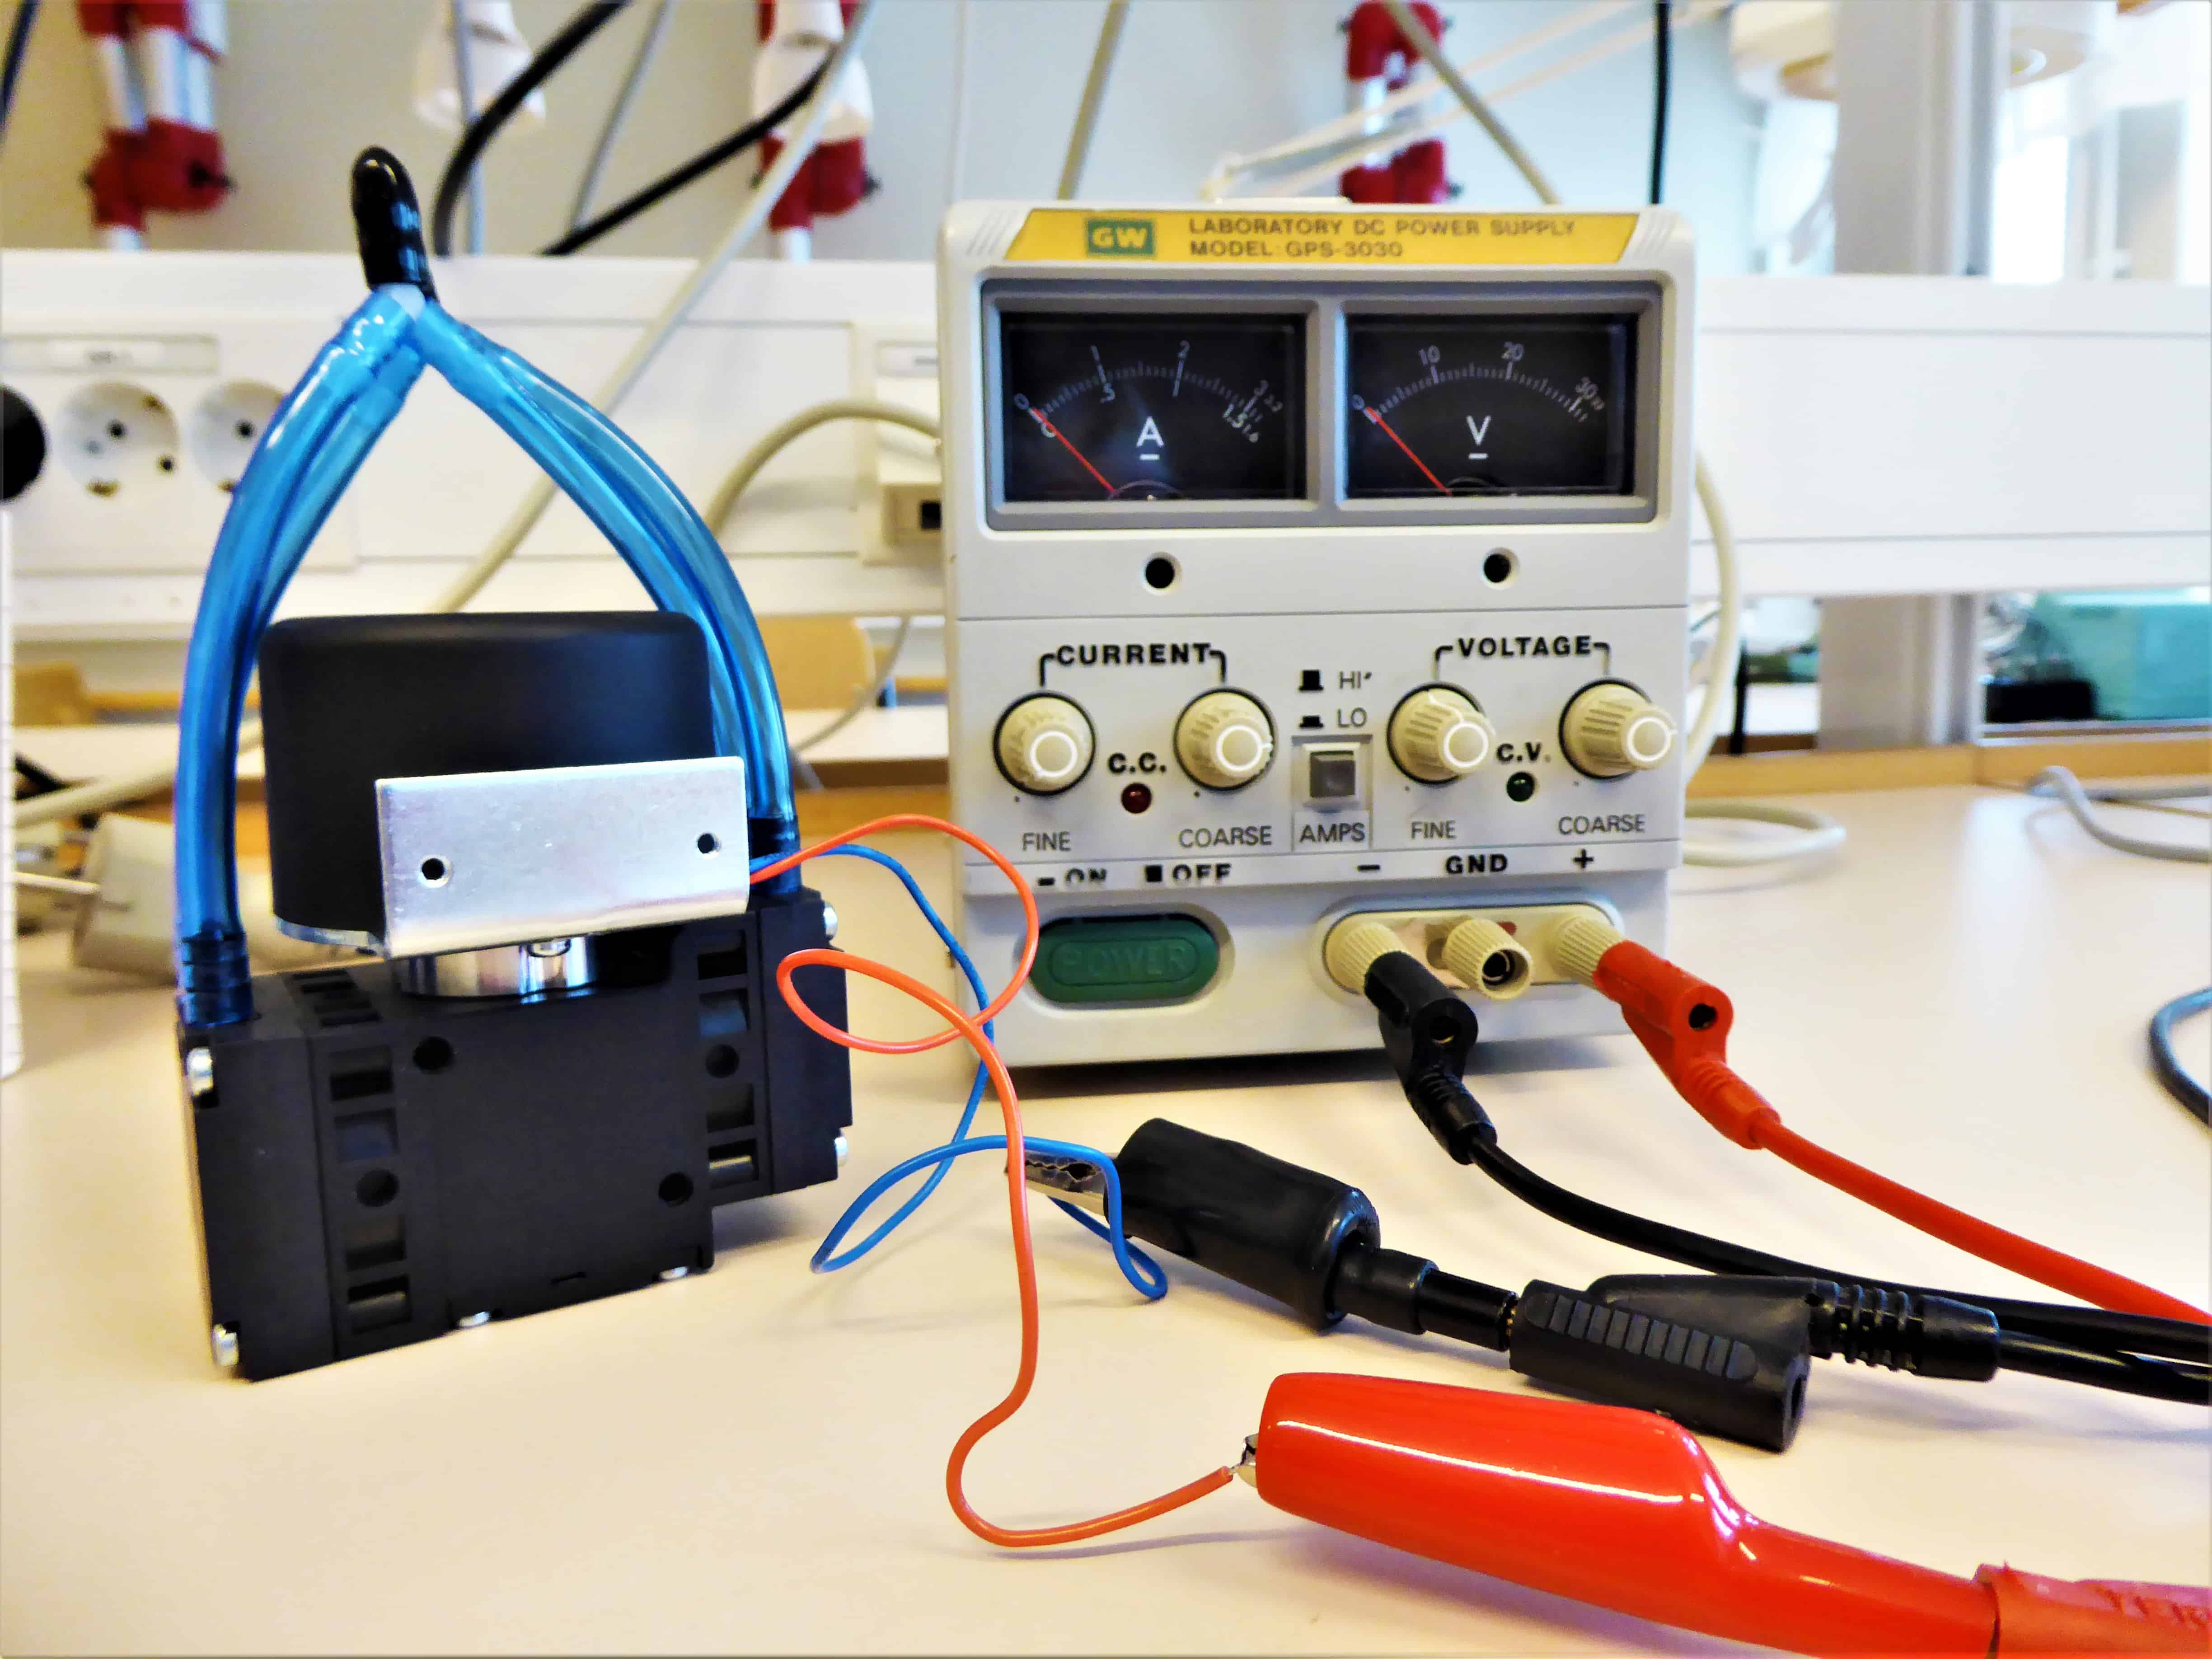
\includegraphics[width=1\linewidth]{5-experiment-verification-and-testing/img/pump-testing.png}
    \end{align*}
    \caption{Photo showing the set-up for the pump testing in the laboratory.} \label{fig:pump-testing}
\end{figure}

\subsubsection{Test 18: Pump Low Pressure}

The pump was tested at low pressure using a small vacuum chamber that is capable of going down to \SI{1}{\hecto\pascal}. For this test the chamber was only taken down to \SI{30}{\hecto\pascal} as this is the expected pressure at 24km, the highest altitude that will be sampled. The experiment set-up can be seen in Figure \ref{fig:pump-low-pressure-set-up}. The pump was connected to the power supply via two cables. It was also screwed into the base plate to prevent it from moving due to its own vibration during the test. A vacuum pump was connected to the chamber wall with a pressure sensor attached to monitor the pressure inside the chamber. 

\begin{figure}[H]
    \begin{align*}
        \includegraphics[width=1\linewidth]{5-experiment-verification-and-testing/img/low-pressure-set-up.png}
    \end{align*}
    \caption {Photo showing the set up of the vacuum chamber, power supply and vacuum pump. }\label{fig:pump-low-pressure-set-up}
\end{figure}

The glass top and cage were then placed on top of the bag and pump and the air slowly removed. Figure \ref{fig:pump-low-pressure-progress} shows the test as it was in progress. 

As the air was removed from the chamber a new problem became immediately obvious. Air that was inside the bag before the test was expanding as the pressure decreased until the bag reached around $75\%$ of its total volume. The air had been pushed out of the sampling bag before the test but this had not been completed thoroughly enough. Therefore care must be taken to ensure that there is no, or very very small amounts, of air inside the bag before it enters a low pressure environment. For subsequent tests the pump was used in reverse to suck any remaining air out of the bags. 

\begin{figure}[H]
    \begin{align*}
        \includegraphics[width=6cm]{5-experiment-verification-and-testing/img/low-pressure-in-progress.png}
    \end{align*}
    \caption {Photo showing the pump and bag in the vacuum chamber during the test.} \label{fig:pump-low-pressure-progress}
\end{figure}

Repeating the test and using the pump to suck out excess air from the bags the chamber was taken to around \SI{30}{\hecto\pascal}. Once the chamber was at this pressure the pump was switched on and a stopwatch began. Once the bag stopped inflating the stopwatch was stopped. During this test there was also a drop in pressure to \SI{28}{\hecto\pascal} and during a repeat there was a drop to \SI{25}{\hecto\pascal}. This also occurred in later tests. This is not seen as a significant problem as during the flight this is exactly what will happen when testing during ascent. In addition the flow rate increases with increasing outside pressure therefore this is showing our worst case flow rate. It was found that the pump was able to successfully switch on and fill the bag at this altitude with a flow rate of approximately 3LPM. 

The test was repeated again at \SI{88}{\hecto\pascal}, representing 17km altitude and \SI{220}{\hecto\pascal}, representing 11km altitude. Here the flow rates were found to be 3.4LPM and 4.9LPM respectively. The results can also be seen in Table \ref{tab:pump-low-pressure-result} and Figure \ref{fig:pump-performance}.

\begin{table}[H]
\centering

\begin{tabular}{|l|l|l|l|l|l}
\cline{1-5}
\textbf{{\small Altitude(km)}}\par & \textbf{{\small Pressure Start(hPa)}}\par & \textbf{{\small Pressure End(hPa)}}\par & \textbf{{\small Time(sec)}}\par & \textbf{{\small Flow Rate(L/min)}}\par &  \\ \cline{1-5}
24 & 30 & 23 & 60 & 3 &  \\ \cline{1-5}
17 & 87 & 80 & 53 & 3.4 &  \\ \cline{1-5}
11 & 220 & 190 & 37 & 4.9 &  \\ \cline{1-5}
\end{tabular}
\caption{Table Showing the Time Taken Until the 3 L Bag Stopped Expanding at Various Different Pressures.}
\label{tab:pump-low-pressure-result}
\end{table}

\raggedbottom

\begin{figure}[H]
    \begin{align*}
        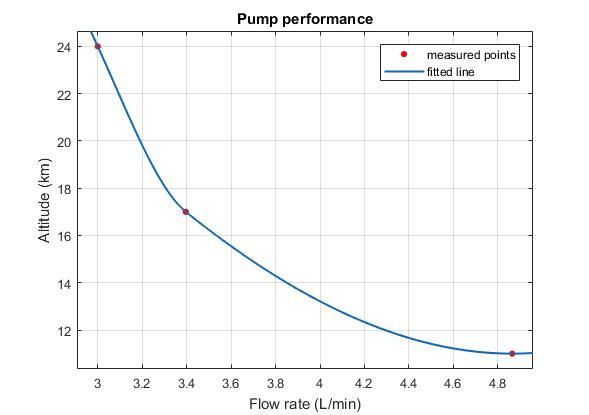
\includegraphics[width=11cm]{5-experiment-verification-and-testing/img/pump-performance.jpg}
    \end{align*}
    \caption {Obtained pump performance at low pressure.} \label{fig:pump-performance}
\end{figure}

\subsubsection{Test 30: Bag Bursting}

A bag was placed in a small vacuum chamber connected to the pump with the same set up as in Test 18, see Figure \ref{fig:pump-low-pressure-set-up} and \ref{fig:pump-low-pressure-progress}. The pump was run for 3 minutes with a full bag to see how the bag reacted. No changes were observed in the bag and no leaks appeared whilst it was in the testing chamber. Upon returning it to atmospheric levels it also appeared to be able to withstand the over pressure. The bag was then left, with the valve closed, on a table where it was handled a little during this time. Approximately 30 minutes after the test the bag made an audible popping noise and air leaked out. The damage that occurred to the bag during the burst can be seen in Figure \ref{fig:bag-burst-front} for the front of the bag and \ref{fig:bag-burst-back} for the back of the bag.

\begin{figure}[H]
    \begin{align*}
        \includegraphics[width=1\linewidth]{5-experiment-verification-and-testing/img/bag-burst-front.png}
    \end{align*}
    \caption {Photo showing the extent of damage on the front of the bag due to bursting.} \label{fig:bag-burst-front}
\end{figure}

\begin{figure}[H]
    \begin{align*}
        \includegraphics[width=1\linewidth]{5-experiment-verification-and-testing/img/bag-burst-back.png}
    \end{align*}
    \caption {Photo showing the extent of damage on the back of the bag due to bursting.} \label{fig:bag-burst-back}
\end{figure}

This kind of bag failure could occur if bags are overfilled, particularly during ascent.

Next the system was set-up in the same way with a new bag. This time the pump was continuously run until failure occured. 

From the damage seen on the bags and from witnessing the burst it can be concluded that if a bag burst during flight it would be highly unlikely to cause damage to any other components on board. The consequences of a single bag burst would be limited to loss of data and a disturbance to audio frequencies. 

\subsubsection{Test 29: Pump Current under Low Pressure}

This test was set up in the same way as above in Test 18, see Figure \ref{fig:pump-low-pressure-set-up} and \ref{fig:pump-low-pressure-progress}. The addition to this test was a multimeter to read the current that the pump was drawing. The pump was tested once with the outlet attached to a bag and once with the outlet sealed. This provides the current when the pump is pumping into an ambient pressure and into a higher pressure.

In general it was found for both cases that decreasing the pressure, or increasing the altitude, lead to a decrease in pump current draw. It was noted that there was an increase in current draw in between sea level conditions and 11km altitude conditions. However as the lowest sampling point it intended to be at 11km this should not be a problem for the experiment. The full results can be seen in Table \ref{tab:pumpcurrentpressure}. 

\begin{table}[H]
\centering

\begin{tabular}{|l|l|l|l|}
\hline
\textbf{Altitude (km)} & \textbf{Pressure (hPa)} & \textbf{Into Bag Current (mA)} & \textbf{Into Seal Current (mA)} \\ \hline
20 & 57 & 140 & 138 \\ \hline
18 & 68 & 150 & 141 \\ \hline
16 & 100 & 161 & 146 \\ \hline
12 & 190 & 185 & 175 \\ \hline
9 & 300 & - & 200 \\ \hline
6 & 500 & - & 242 \\ \hline
0 & 1013 & - & 218 \\ \hline
\end{tabular}
\caption{Table Showing How the Current Draw of the Pump Changed With Outside Air Pressure for Two Different Conditions. The First Pumping Into a Sampling Bag and the Second Pumping Into a Sealed Tube.}
\label{tab:pumpcurrentpressure}
\end{table}

A graphical representation of these results are shown in Figures \ref{fig:pumpcurpresbag} and \ref{fig:pumpcurpres}. From the table and figures it can be seen that the current draw is higher during the bag filling than during the sealed case. As the experiment will sample between 11km and 24km it can be concluded that the highest current draw will occur during the 11km altitude sample and can be expected to be around 200mA. 

\begin{figure}[H]
    \begin{align*}
        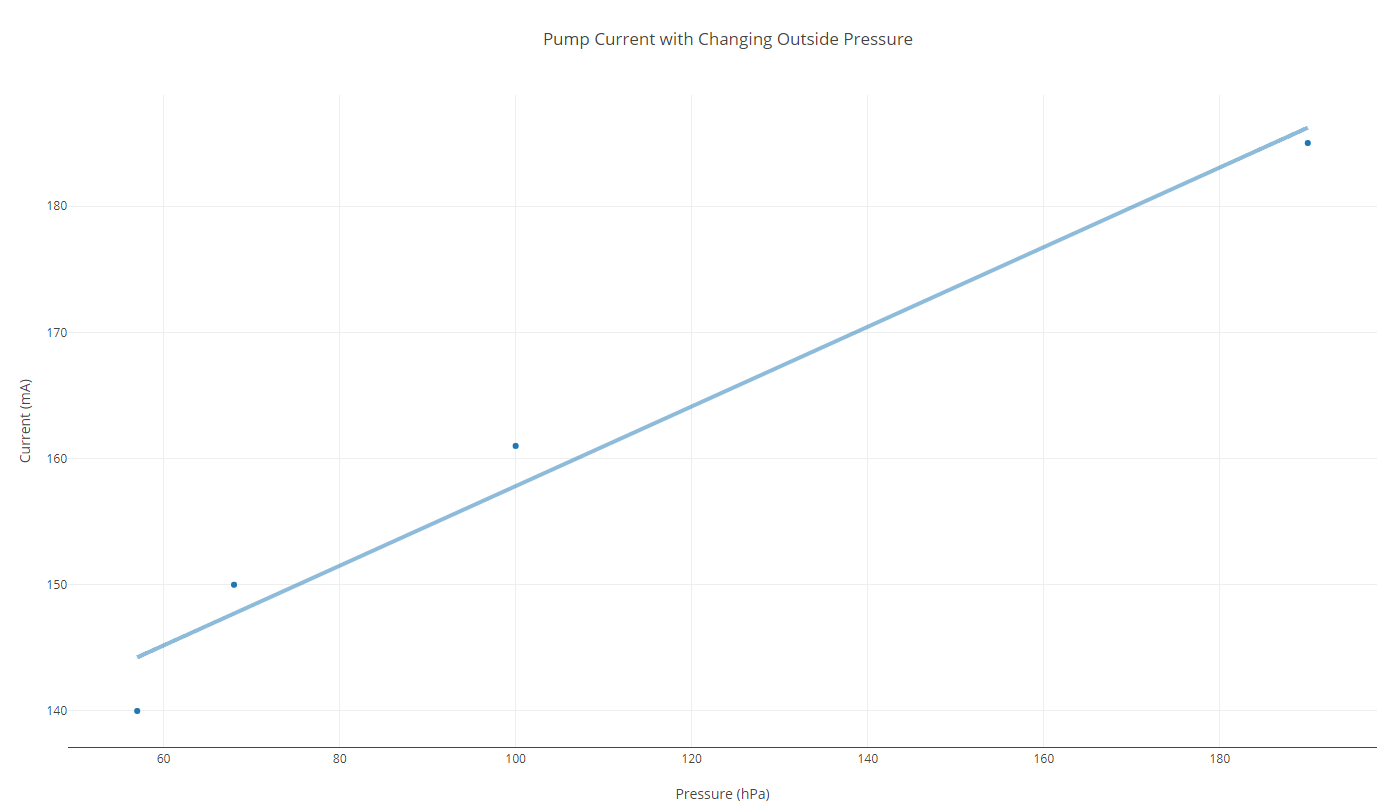
\includegraphics[width=1\linewidth]{5-experiment-verification-and-testing/img/pump-cureent-pressure.png}
    \end{align*}
    \caption {Graph showing the expected current values when the pump is pumping air into a a bag based upon the results obtained.} \label{fig:pumpcurpresbag}
\end{figure}


\begin{figure}[H]
    \begin{align*}
        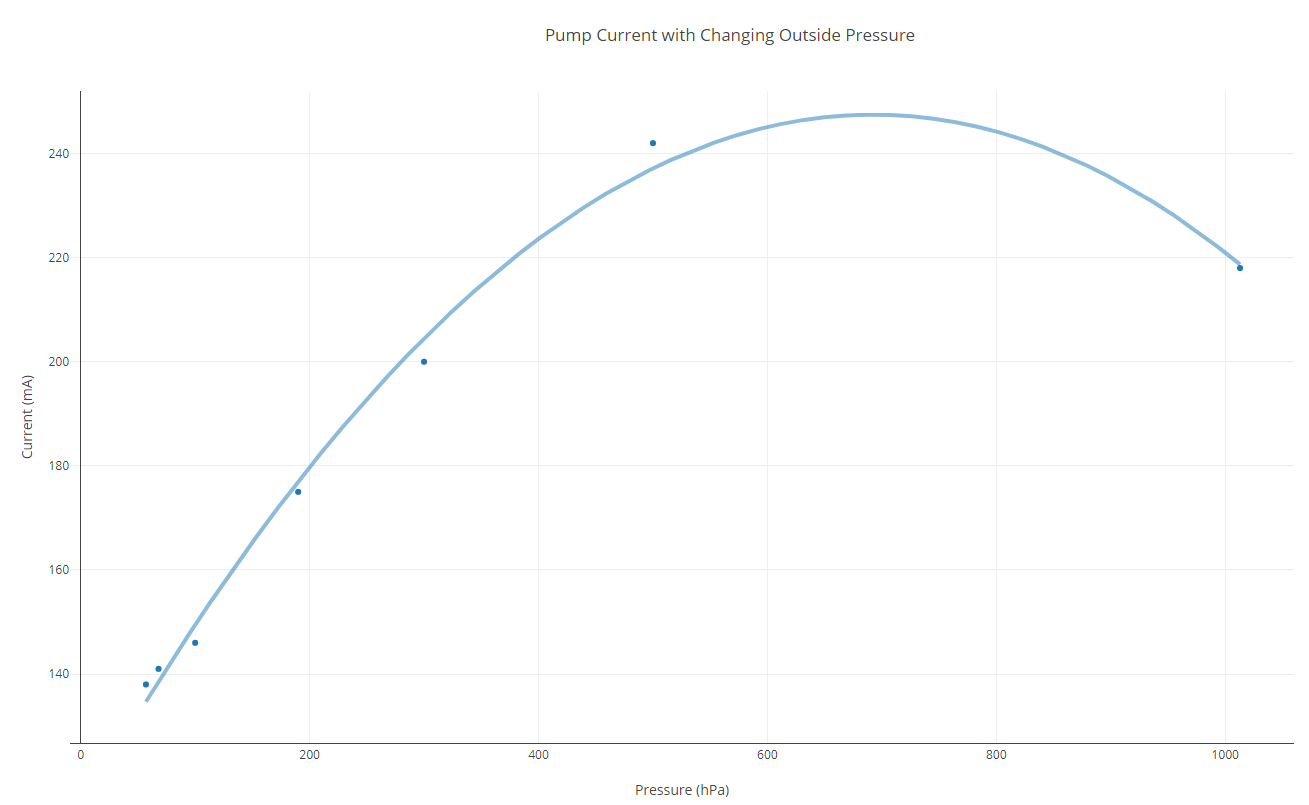
\includegraphics[width=1\linewidth]{5-experiment-verification-and-testing/img/pump-current-pressure.png}
    \end{align*}
    \caption {Graph showing the expected current values when the pump is pumping air into a sealed outlet based upon the results obtained and the data shown in Figure \ref{fig:pumpflowcur}.} \label{fig:pumpcurpres}
\end{figure}

By looking at the data from both Test 18 and Test 29 a relationship can be seen between the outside air pressure, the flow rate of the pump and the current draw of the pump. 

\subsubsection{Test 17: Bags' holding times and samples' condensation verification}


This test was realized at the Finish Metereological Institute in Sodankyl\"{a}. Eight Multi-Layer Foil bags of 1L volume were connected to SMC valves and all together connected in series with stainless steel tubes. 

\begin{figure}[H]
    \begin{align*}
        \includegraphics[width=1\linewidth]{5-experiment-verification-and-testing/img}
    \end{align*}
    \caption {Graph showing the expected current values when the pump is pumping air into a sealed outlet based upon the results obtained and the data shown in Figure \ref{fig:pumpflowcur}.} \label{fig:pumpcurpres}
\end{figure}


\begin{figure}[H]
    \begin{align*}
        \includegraphics[width=1\linewidth]{5}
    \end{align*}
    \caption {Graph showing the expected current values when the pump is pumping air into a sealed outlet based upon the results obtained and the data shown in Figure \ref{fig:pumpflowcur}.} \label{fig:pumpcurpres}
\end{figure}


\begin{figure}[H]
    \begin{align*}
        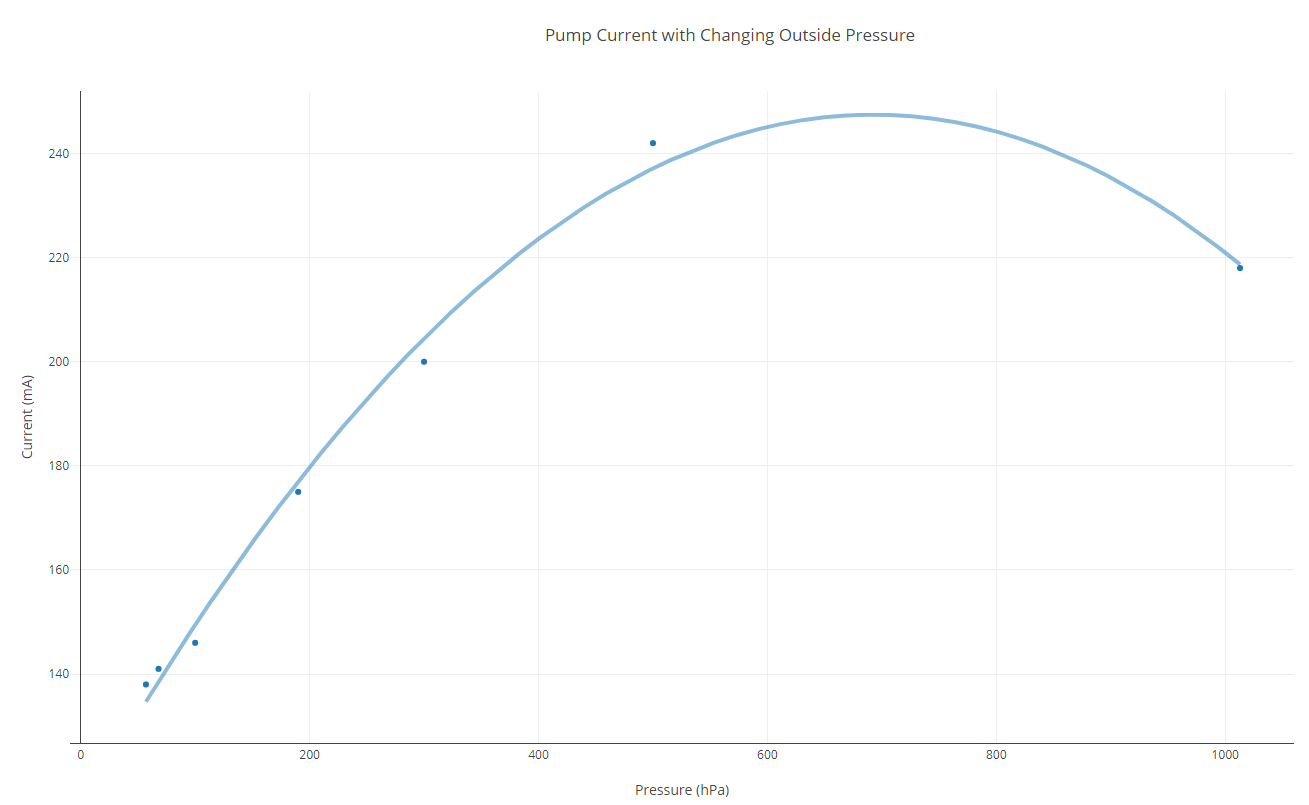
\includegraphics[width=1\linewidth]{5-experiment-verification-and-testing/img/pump-current-pressure.png}
    \end{align*}
    \caption {Graph showing the expected current values when the pump is pumping air into a sealed outlet based upon the results obtained and the data shown in Figure \ref{fig:pumpflowcur}.} \label{fig:pumpcurpres}
\end{figure}
% est  procedure:   All  valves,  bags  and  tubes  must  be  connected.Then  the  entire  system  needs  to  be  flushed  the  same  way  it  willbe  for  the  flight.   After  flushing  the  bags  will  then  be  filled  witha gas of known concentration.  The bags will then be left outsidefor  6,  12,  24  and  48  hours.  Using  8  bags  in  total  with  two  bagsfor each time duration.  After each time duration two bags will beremoved and analysed using the picarro analyser.  The concentra-tion of gases found inside the bags will be compared to the initialconcentration  of  the  air  placed  in  the  bags.  If  the  concentrationchanges then the bags must be retrieved and analysed before thatamount of time has elapsed for the samples to beTest duration:  3 days.